\section{Playing the traverse game over Karstaway}
 \margininbox{Electric Dreams}{
     \begin{citemize}
    \item Jack Hare
    \item Dave Wilson II
    \item Rhys Tyers
    \end{citemize}}{\explo}
    
\subsection{Electric Dreams}

My favourite pushing trip of 2016 was \passage{Karstaway}, a 30\,m undescended shaft left unexplored by the JSPDT \sidenote{Due to some confusion at the time of pushing, we called it \protect\passage{Karstaway} pitch, it had been surveyed previously as \protect\passage{Rokovo Brezno}, the name which appears on the survey} which yielded a huge amount of passage and a connection into the \passage[branch]{TTT} branch. But the survey showed that the Slovenians had actually passed over the top of this pitch and into passage beyond. They left more undropped shafts, but they were sure it connected into \passage[branch]{TTT}.


\begin{marginfigure}
\centering
\frame{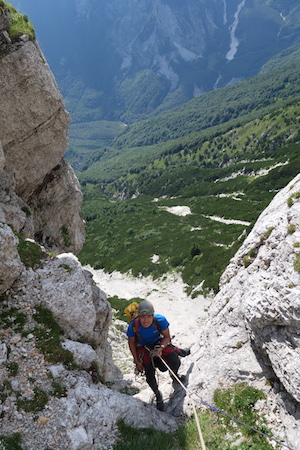
\includegraphics[width=\textwidth]{images/2017/jack-electric-2017/kenneth-abseil.jpg}}
\caption{Early on in the 2017 expedition, a rebolting project for the surface abseil to \protect\passage[abseil]{Primadona} took place; here Kenneth Tan takes down a tackle sack of new 11mm rope for the job \pic{Rhys Tyers}}
\label{kenneth abseil}
\end{marginfigure}


I identified Davie Dubz as a man who would enjoy sitting around for hours whilst I bolted a route up above the huge pitch. Equipped with drills and rope, we set off down to the pitch head, and I helpfully pointed out facts and cave trivia to Davie, like where Arun and Will waited for rescue last year.

At the pitch head, I was suddenly unsure. The drop is large, and there was no obvious way up over it. Surely the Slovenians hadn't just free climbed over a 40\,m drop (they had done just this, it turned out.) I back tracked, found part of the rift that I could free climb up in, and began placing bolts. First I dropped a rope for Davie, who joined me on the upper level. He dug a small hollow in the soft mud and lowered himself into it for warmth, pronouncing himself completely content. I began to bolt.

The first few were easy, with passable foot holds as the false floor dropped away. Then I encountered a huge slab wedged in the passage. Careful inspection showed that the left wall was also about to flake away, so I carefully crawled over the wedge boulder, bolting only on the right wall. After this I regained a false floor with no way on but a pitch down. Dropping this pitch a few metres landed me in a small chamber, containing a rusted steel bolt.

The Slovenians had been here, and I could see the pitch head of \passage{Karstaway} through a hole in the floor. Concious that the entire floor was probably just propped boulders, I placed a new bolt in this chamber, put the rope in and then abseiled down to \passage{Karstaway} pitch head.

Now I had a problem - my rope started all the way back in the bottom of the rift, but I needed to derig it all without stranding myself or Davie. After significant thought, I worked it all out, and chopped the rope at the right point before derigging back into the rift above \passage{Karstaway}. 

The trip had taken the whole day, I waste twelve lovely new stainless steel bolts that will never be used again, but we had done it - the way into the route over \passage{Karstaway} was done. We had walked down the good sized passage until the next pitch, then turned round and headed to the surface, excited to (re-)find a storming lead.

\begin{figure*}[t!]
\checkoddpage \ifoddpage \forcerectofloat \else \forceversofloat \fi
\centering
\frame{\includegraphics[width=\textwidth]{"images/2017/jack-electric-2017/electric-dreams-2".jpg}}
\caption{Jack Hare and Dave `Davie Dubz' Wilson at the bottom of the \protect\passage{Electric Dreams} main pitch \pic{Rhys Tyers}}
\label{Elec dreams main pitch}
\end{figure*}

The next trip Rhys opted to join us, lured by promises of 500\,m of good walking passage and equipped with his photography kit. Davie rigged the first pitch, a steep slope covered in loose rock. At the bottom was a tight, tall rift full of sharp rock that gripped and tore at our oversuits. I swung blindly with the bolting hammer, clearing the way as we advanced, cursing all the rope we had with us. I spotted a few boot prints deep in the mud underwater, proof we were merely retracing the steps of others.

Soon we came to a pitch - just a short one mind, but far too deep to free climb, and I perked up at the prospect of finding something new. A Y-hang got me down five metres to a chamber split in two by a large rift. Cautiously I approached, then whooped at the size of the shaft below. I bolted an epic Y-hang on opposite walls (a signature rigging piece, qv. \passage{Hall of the Mountain King}) and dropped down to a ledge which contained a large, crystal clear pool.

Rhys and Davie soon joined me, and I stranded them on this ledge as I swung out to drop the rest of the shaft. Davie tried to push a tight phreatic tube behind the lake, but couldn't quite fit, and soon they joined me in the good size, flat bottom chamber at the bottom of the shaft. Lots of water flowed down into this chamber, and one entire wall was missing, leading only into the void.


\begin{marginfigure}
\checkoddpage \ifoddpage \forcerectofloat \else \forceversofloat \fi
\centering
\frame{\includegraphics[width=\linewidth,]{"images/2017/jack-electric-2017/dave-crystal_pool".jpg}}
\caption{Jack Hare and Dave `Davie Dubz' Wilson at the bottom of the \protect\passage{Electric Dreams} main pitch \pic{Rhys Tyers}}
\label{Crystal pool}
\end{marginfigure}

Rhys took over bolting here, and quick made it out onto a ledge overlooking a large chamber, \bignote{with plentiful leads at every level}. He rigged down, and we dropped into the boulder floored chamber. After quickly checking out a grim looking lead in the floor, we took the obvious way on at the far side of the chamber, through a winding, walkable rift. At the far end we found only darkness - another vast chamber.

\begin{figure*}[t!]
\checkoddpage \ifoddpage \forcerectofloat \else \forceversofloat \fi
\centering
\frame{\includegraphics[width=\linewidth]{"images/2017/jack-electric-2017/electric_dreams".jpg}}
\caption{Dave Wilson standing over the clear pool attempts to push a very tight rift \pic{Rhys Tyers}}
\end{figure*}

The day spent rigging the traverse was worth-while, and we photographed our great find as we prussiked out. In honour of our recent brush with lightning, we named it `\passage{Electric Dreams}'. 

\subsection{Strangehold}
The lure of \passage{Electric Dreams} was strong, and soon Davie and I returned. The rift crawl didn't seem as tough this time, and we were soon down in the large chamber. Turning to Davey, I asked a question I instantly regretted - `Which lead do you want to push first?' Instead of opting for the obvious vast chamber down the walking size rift, he plumbed for the tight, scrotty hole in the floor. `When it dies, we can push the nice lead.' he offered, pragmatically.

\margininbox{Stranglehold}{
     \begin{citemize}
    \item Jack Hare
    \item Dave Wilson II
    \end{citemize}}{\explo}

\begin{survey}[b!]
\checkoddpage \ifoddpage \forcerectofloat \else \forceversofloat \fi
\frame{\includegraphics[width=\linewidth]{"images/2017/jack-electric-2017/electricdreamsee".png}}
\caption[Extended Elevation of Electric Dreams series]{Extended Elevation of Electric Dreams series \pen{Jack Hare, bivi logbook}}
\end{survey}

One short handline later, we were into anstreamway of brown, fragile rock that enjoyed breaking off then stabbing you in the knee. Davey enjoyed himself immensely, and gave up several times before I pointed out bypasses to the various sumps and ducks. After much thrutching, we broke out into a small pitch which I inadvisably free climbed before going back for the drill.

To keep Davey warm, I set him off putting up survey cairns for the way back out. I was soon down at the bottom of a shaft that broke into a narrow, hading rift. \bignote{Davey joined me, and we soon realised the rift was too tight for any progress}. Fortunately there was a phreatic tube a metre or so off the floor, and after crawling through this we broke out above the rift.

The draft was strong, and the rift opened into a boulder collapse chamber, entered via a short free climb down. I was quite sketched out when I got down - huge stacked boulders, seemingly unsupported and ready to fall, so I asked Davey to stay put whilst I checked it out. I hurriedly looked into every likely lead, but they were all too tight and too sketchy. We back tracked, and named our find `\passage{Stranglehold}' - a phreatic tube ended by a choke.

Not ready to be done yet, I realised that the passage continued on the other side at the top of the shaft. I hastily converted the long hang into a very silly swing pitch (2\,m down, 5\,m sideways…) \sidenote{Note of the editor: the eventual connection of \protect\passage{Stranglehold} with the \protect\passage{Hall of the Mountain King} cancelled the need for this obstacle} and reached the passage on the other side. The passage was tight and sharp, but dry. We free climbed a few drops that we later put handlines on, and squeezed and grovelled through some tight bits.

At the bottom of short pitch I tapped a blade of rock with my foot as I climbed down. \bignote{It rang out with a perfect, clear note that took a long time to die away - a natural tuning fork}, formed by nature, and found by us. Only Tanguy has also heard it, so that's three people in the world. Such events are the true beauty of cave exploration.

Onwards, and we broke out into a huge rift. We arrived at the top of a large pile of rocks, and after bolting a traverse down some of the way I backtracked and began to garden. Using my feet (steel toe capped wellies are great) I progressively eroded the slope of very loose, large rocks over the course of thirty minutes. Davey gawped at the noise and the sight of so many rocks disappearing down the rift below.

Eventually I was happy to continue down. There were huge wedged boulders the size of houses on either side, but I tried to find some true wall in which to place my bolts. One good Y-hang and I started down. Soon I realised the size of this rift - at least thirty or so metres down, and reminiscent of \passage{Hall of the Mountain King}, which I'd also found last year. But I could see no familiar markers to confirm that it was \passage{HotMK}, and as I descended I became more sure it was somewhere new.

\begin{marginsurvey}
\checkoddpage \ifoddpage \forcerectofloat \else \forceversofloat \fi
\centering
 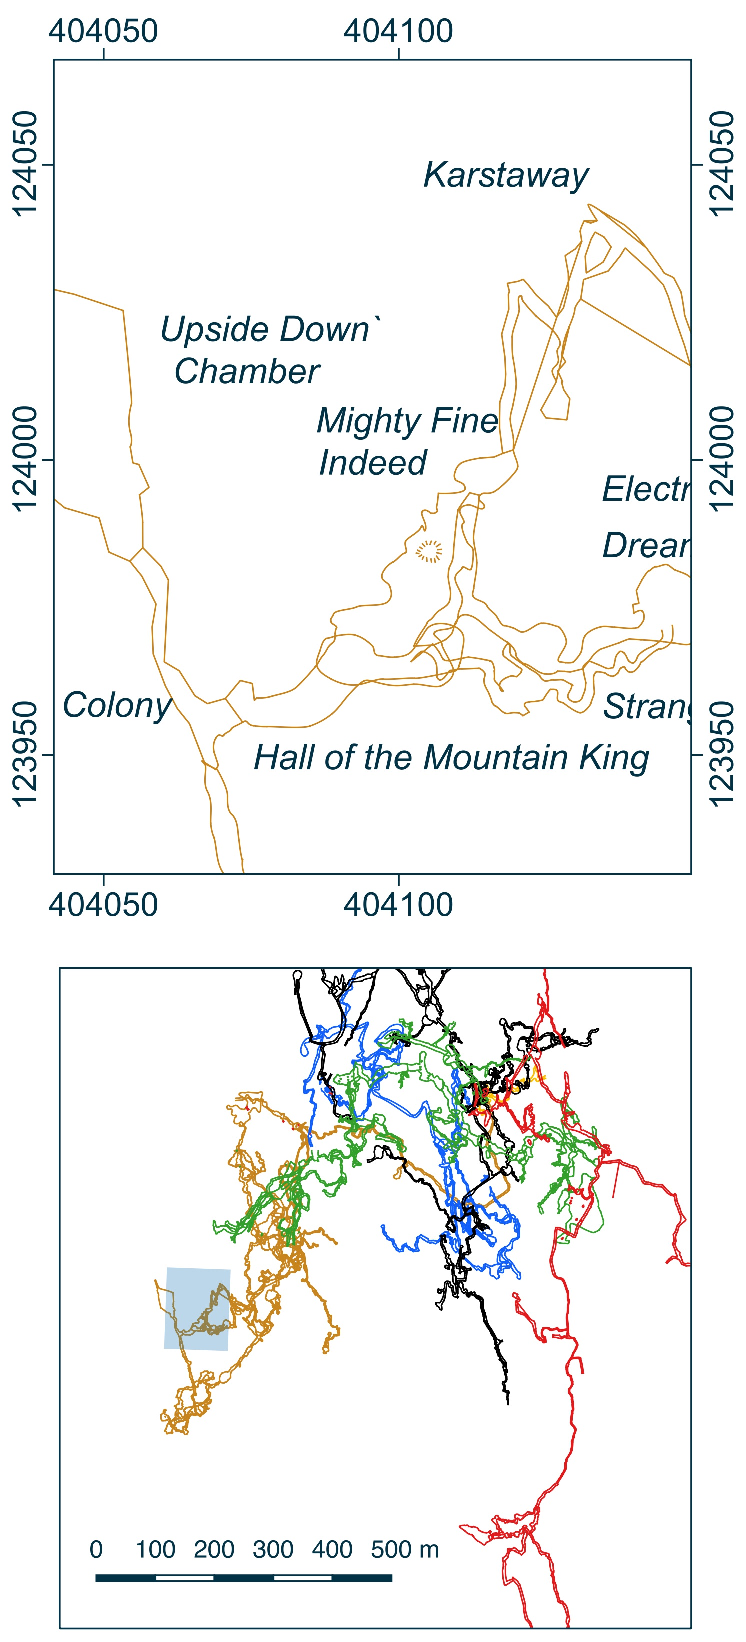
\includegraphics[width=\linewidth]{images/little_insets/hotmk_inset.pdf}
 \caption[Electric Dreams]{Plan view of the Electric Dreams and Stranglehold extensions over the top of the \protect\passage{Hall of the Mountain King}. Slovenian National Grid ESPG 3794}
 \label{Mountain King inset 2}
\end{marginsurvey}

The rope began to twang above me, never a good noise when you're dangling some ten metres above the ground. I looked around for somewhere to put a deviation, out of bolts and maillons. I spent some time swinging around before I realised I was too tired, and too freaked out to continue. 

Reluctantly, I dropped my rope to the bottom to check it could reach, and then prussiked out, leaving it there. I figured if it was \passage[|see{Hall of the Mountain King}]{Hall of the Mountain King} then someone else might find it there and confirm where I'd dropped into\sidenote{This intuition was nearly correct, as \passage{Hall of the Mountain King} was accessed from the next pitch down.}.

Reunited with a very cold David, we began to survey out. It took a very long time, and David's survey station placement near the end left something to be desired. I taught him a few tricks to speed things up, and finally we were done.

As we hurried out of the cave, I realised we would miss our call out. I was furious with myself, as I was always hard on others who did that. I pushed myself as hard as I could to get to the surface, my vision swimming and head pounding as I prussiked up the cliff abseil. DW saw our lights at 9:58\,pm, effectively cancelling our call out with two minutes to go.

Back at the bivi \bignote{I collapsed, lying on the floor until someone shoved a mess tin my way}. I ate mechanically until I'd recovered enough to tell the others (worried at my uncharacteristically quiet state) what we'd found. Probably my best pushing trip of 2017, and props to Davey for choosing to push the shit lead.

\name{Jack Hare}
